\chapter{Análisis del sistema}
\label{ch:analisis}
En este capítulo se formalizará de qué será capaz el producto desarrollado. Comienza con una descripción del sistema de una manera más detallada, después se extraerán los casos de uso y requisitos de usuario, que nos permiten hacernos a la idea de lo que necesita el sistema y poder conceptualizarlo en forma de requisitos de software. En último lugar se establecerá la relación entre los requisitos de usuario y los de software en una matriz de trazabilidad, que nos permiten comprobar que todo lo que el usuario ha pedido ha sido tenido en cuenta.

Además este capítulo sirve como base para los siguientes capítulos, Diseño e Implementación, en los que basándose en los requisitos recogidos se empezara a dar vida al sistema.

\section{Definición del Sistema}
El propósito del proyecto es desarrollar un dispositivo que nos proporcione videovigilancia y medidas de diferentes factores, para garantizar la seguridad de un CPD. Las diferentes medidas que se tomen se almacenaran para poder ser consultadas junto con la imagen de videovigilancia a través de una plataforma web.
\begin{figure}[H]
	\ffigbox[\FBwidth]
	{\caption{Diagrama del sistema}}
	{\tikzset{every picture/.style={line width=0.75pt}} %set default line width to 0.75pt        

    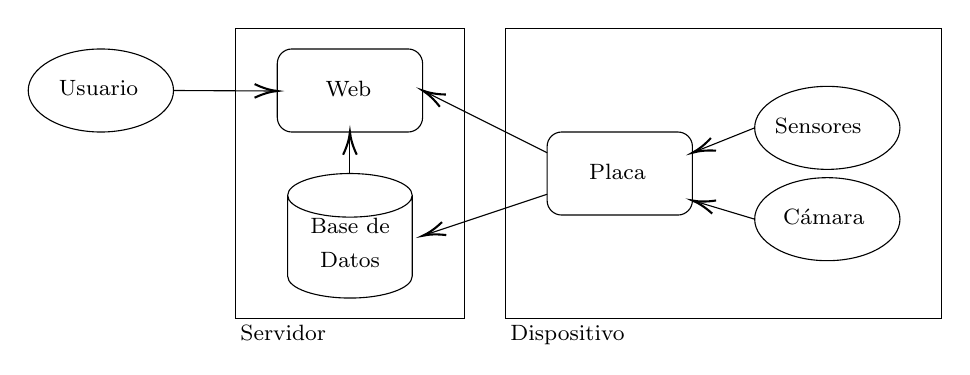
\begin{tikzpicture}[x=0.75pt,y=0.75pt,yscale=-1,xscale=1]
    %uncomment if require: \path (0,300); %set diagram left start at 0, and has height of 300
    
    %Shape: Ellipse [id:dp09985323197995077] 
    \draw   (90,90) .. controls (90,78.95) and (105.67,70) .. (125,70) .. controls (144.33,70) and (160,78.95) .. (160,90) .. controls (160,101.05) and (144.33,110) .. (125,110) .. controls (105.67,110) and (90,101.05) .. (90,90) -- cycle ;
    
    %Flowchart: Process [id:dp27577112697014905] 
    \draw   (320,60) -- (530,60) -- (530,200) -- (320,200) -- cycle ;
    %Shape: Ellipse [id:dp8579510276491811] 
    \draw   (440,108) .. controls (440,96.95) and (455.67,88) .. (475,88) .. controls (494.33,88) and (510,96.95) .. (510,108) .. controls (510,119.05) and (494.33,128) .. (475,128) .. controls (455.67,128) and (440,119.05) .. (440,108) -- cycle ;
    
    %Flowchart: Magnetic Disk [id:dp5977420418153743] 
    \draw   (275,140.5) -- (275,179.5) .. controls (275,185.3) and (261.57,190) .. (245,190) .. controls (228.43,190) and (215,185.3) .. (215,179.5) -- (215,140.5)(275,140.5) .. controls (275,146.3) and (261.57,151) .. (245,151) .. controls (228.43,151) and (215,146.3) .. (215,140.5) .. controls (215,134.7) and (228.43,130) .. (245,130) .. controls (261.57,130) and (275,134.7) .. (275,140.5) -- cycle ;
    
    %Flowchart: Alternative Process [id:dp8760474928959088] 
    \draw   (210,77) .. controls (210,73.13) and (213.13,70) .. (217,70) -- (273,70) .. controls (276.87,70) and (280,73.13) .. (280,77) -- (280,103) .. controls (280,106.87) and (276.87,110) .. (273,110) -- (217,110) .. controls (213.13,110) and (210,106.87) .. (210,103) -- cycle ;
    
    %Flowchart: Alternative Process [id:dp21352688625982807] 
    \draw   (340,117) .. controls (340,113.13) and (343.13,110) .. (347,110) -- (403,110) .. controls (406.87,110) and (410,113.13) .. (410,117) -- (410,143) .. controls (410,146.87) and (406.87,150) .. (403,150) -- (347,150) .. controls (343.13,150) and (340,146.87) .. (340,143) -- cycle ;
    
    %Shape: Ellipse [id:dp26663174856799987] 
    \draw   (440,152) .. controls (440,140.95) and (455.67,132) .. (475,132) .. controls (494.33,132) and (510,140.95) .. (510,152) .. controls (510,163.05) and (494.33,172) .. (475,172) .. controls (455.67,172) and (440,163.05) .. (440,152) -- cycle ;
    
    %Straight Lines [id:da29668504082176317] 
    \draw    (440,152) -- (411.92,143.57) ;
    \draw [shift={(410,143)}, rotate = 376.7] [color={rgb, 255:red, 0; green, 0; blue, 0 }  ][line width=0.75]    (10.93,-3.29) .. controls (6.95,-1.4) and (3.31,-0.3) .. (0,0) .. controls (3.31,0.3) and (6.95,1.4) .. (10.93,3.29)   ;
    %Straight Lines [id:da24405119567314104] 
    \draw    (440,108) -- (411.86,119.26) ;
    \draw [shift={(410,120)}, rotate = 338.2] [color={rgb, 255:red, 0; green, 0; blue, 0 }  ][line width=0.75]    (10.93,-3.29) .. controls (6.95,-1.4) and (3.31,-0.3) .. (0,0) .. controls (3.31,0.3) and (6.95,1.4) .. (10.93,3.29)   ;
    %Straight Lines [id:da573358835450916] 
    \draw    (160,90) -- (208,90.24) ;
    \draw [shift={(210,90.25)}, rotate = 180.29] [color={rgb, 255:red, 0; green, 0; blue, 0 }  ][line width=0.75]    (10.93,-3.29) .. controls (6.95,-1.4) and (3.31,-0.3) .. (0,0) .. controls (3.31,0.3) and (6.95,1.4) .. (10.93,3.29)   ;
    %Straight Lines [id:da7053149916028076] 
    \draw    (340,120) -- (281.79,90.89) ;
    \draw [shift={(280,90)}, rotate = 386.57] [color={rgb, 255:red, 0; green, 0; blue, 0 }  ][line width=0.75]    (10.93,-3.29) .. controls (6.95,-1.4) and (3.31,-0.3) .. (0,0) .. controls (3.31,0.3) and (6.95,1.4) .. (10.93,3.29)   ;
    %Straight Lines [id:da758134561546915] 
    \draw    (340,140) -- (281.9,159.37) ;
    \draw [shift={(280,160)}, rotate = 341.57] [color={rgb, 255:red, 0; green, 0; blue, 0 }  ][line width=0.75]    (10.93,-3.29) .. controls (6.95,-1.4) and (3.31,-0.3) .. (0,0) .. controls (3.31,0.3) and (6.95,1.4) .. (10.93,3.29)   ;
    %Straight Lines [id:da833678135330659] 
    \draw    (245,130) -- (245,112) ;
    \draw [shift={(245,110)}, rotate = 450] [color={rgb, 255:red, 0; green, 0; blue, 0 }  ][line width=0.75]    (10.93,-3.29) .. controls (6.95,-1.4) and (3.31,-0.3) .. (0,0) .. controls (3.31,0.3) and (6.95,1.4) .. (10.93,3.29)   ;
    %Flowchart: Process [id:dp23665676445923722] 
    \draw   (190,60) -- (300,60) -- (300,200) -- (190,200) -- cycle ;
    
    % Text Node
    \draw (321,202) node [anchor=north west][inner sep=0.75pt]  [font=\footnotesize] [align=left] {Dispositivo};
    % Text Node
    \draw (222,150.43) node [anchor=north west][inner sep=0.75pt]   [align=left] {\begin{minipage}[lt]{32.67pt}\setlength\topsep{0pt}
    \begin{center}
    {\footnotesize Base de}\\{\footnotesize Datos}
    \end{center}
    
    \end{minipage}};
    % Text Node
    \draw (232,84) node [anchor=north west][inner sep=0.75pt]  [font=\footnotesize] [align=left] {Web};
    % Text Node
    \draw (191,202) node [anchor=north west][inner sep=0.75pt]  [font=\footnotesize] [align=left] {Servidor};
    % Text Node
    \draw (103.5,84) node [anchor=north west][inner sep=0.75pt]  [font=\footnotesize] [align=left] {Usuario};
    % Text Node
    \draw (359,124) node [anchor=north west][inner sep=0.75pt]  [font=\footnotesize] [align=left] {Placa};
    % Text Node
    \draw (448.5,102) node [anchor=north west][inner sep=0.75pt]  [font=\footnotesize] [align=left] {Sensores};
    % Text Node
    \draw (452.5,146) node [anchor=north west][inner sep=0.75pt]  [font=\footnotesize] [align=left] {Cámara};
    
    
    \end{tikzpicture}}
\end{figure}

Como se puede ver en el diagrama el sistema consistirá en una página web alojada en nuestro servidor, que también dispondrá de una base de datos para almacenar toda la información necesaria para el funcionamiento del sistema. La web podrá ser accedida por el usuario, que en este caso será el personal encargado del control de esa sala CPD Por otro lado tenemos la parte del dispositivo que consta de una placa que recibe medidas a través de una serie de sensores y un cámara que actuará como cámara de videovigilancia. La placa enviara las medidas a la base de datos donde ser almacenaran junto a la información del dispositivo y dará acceso a la imagen de la cámara mediante la web.

\section{Casos de uso}
Se presenta a continuación un diagrama que resume todos los casos de uso del sistema.

DIAGRAMA

Para realizar una descripción más detallada de los casos de uso emplearemos la representación tabular que se muestra en la siguiente plantilla.
\begin{table}[H]
    \centering
    \caption{Plantilla de Caso de Uso}
    \begin{tabular}{|l|l|}
    \hline
    \multicolumn{2}{|c|}{\cellcolor[HTML]{BFBFBF}{\color[HTML]{000000} \textbf{CU-XX}}} \\ \hline
    \textbf{Caso de uso} & $\quad\quad\quad\quad\quad\quad\quad\quad\quad\quad$ \\ \hline
    \textbf{Actores} &  \\ \hline
    \textbf{Descripción} &  \\ \hline
    \textbf{Precondiciones} &  \\ \hline
    \textbf{Postcondiciones} &  \\ \hline
    \end{tabular}
\end{table}

\begin{itemize}
    \item \textbf{CU-XX:} Identificador del caso de uso, el XX tomará un valor en función del orden de este.
    \item \textbf{Caso de uso:} Nombre que identifica el caso de uso.
    \item \textbf{Actores:} Partes implicadas en el caso de uso.
    \item \textbf{Descripción:} Breve exposición de la situación.
    \item \textbf{Precondiciones:} Condiciones que se deben cumplir para que tenga lugar.
    \item \textbf{Postcondiciones:} Que tiene lugar si se da el caso de uso.
\end{itemize}

Ahora que entendemos el significado de cada una de las casillas procedemos a detallar los casos de uso.

\section{Requisitos de usuario}

\section{Requisitos de software}

\section{Matriz de trazabilidad}